\documentclass{beamer}
\usepackage[utf8]{inputenc}
\usetheme{default}
\usecolortheme{dove}
\usepackage{textpos}
\usepackage{grid-system}

% po4a: environment frame
% po4a: environment Row
% po4a: environment Cell


\title{Strategic Plan for World Domination}
\author{
\includegraphics[width=8cm]{Cat_in_Tank}} %\\ \tiny{src: id\_iom.deviantart.com}} %src: id_iom.deviantart.com
%\institute[Inst.]{Freifunk Darmstadt}
\date{}

\begin{document}

\begin{frame}
\maketitle
\end{frame}

\addtobeamertemplate{frametitle}{}{%
\begin{textblock*}{100mm}(0.93\textwidth,-0.5cm)

\includegraphics[height=1cm]{logo} 
\end{textblock*}}

%\begin{frame}{Outline}
%\tableofcontents
%\end{frame}

\section{Current scenario}
\begin{frame}{Current status}
\vfill
\begin{center}
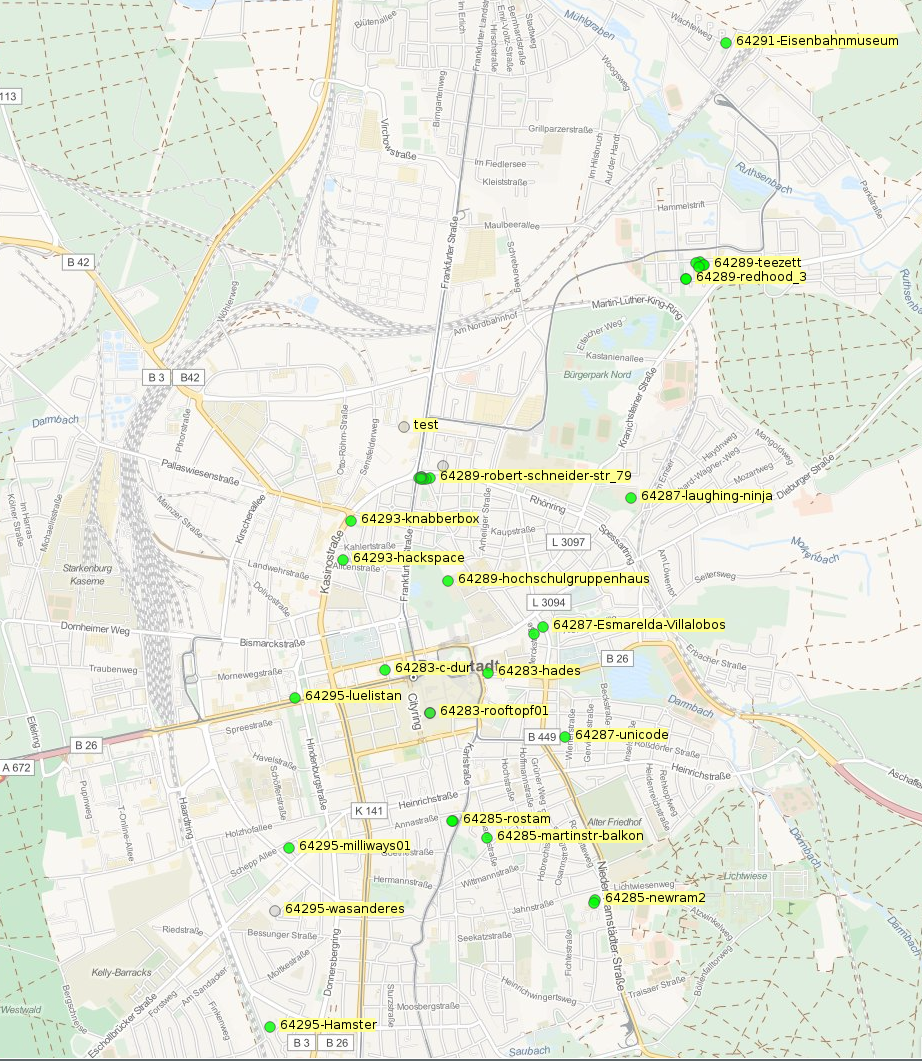
\includegraphics[height=0.8\textheight]{darmstadt-map}
\end{center}
\end{frame}

\section{How can we develop the network}
\begin{frame}{How can we develop the network}
\vfill
from this...\\
\begin{center}
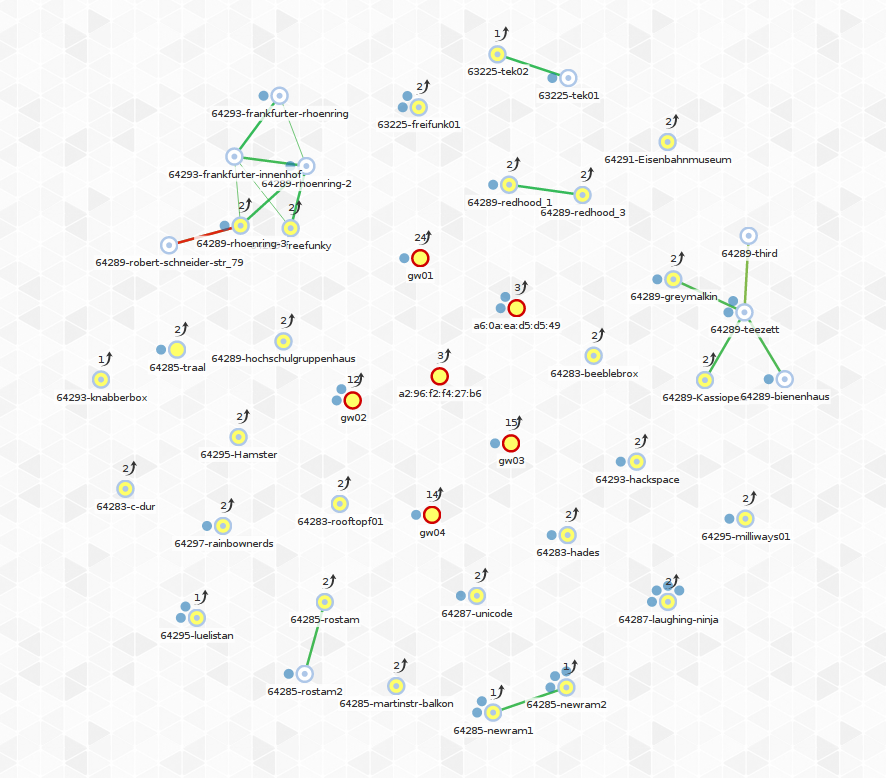
\includegraphics[height=0.8\textheight]{darmstadt-graph}
\end{center}
\end{frame}

\begin{frame}{How can we develop the network}
\vfill
to this?\\
\begin{center}
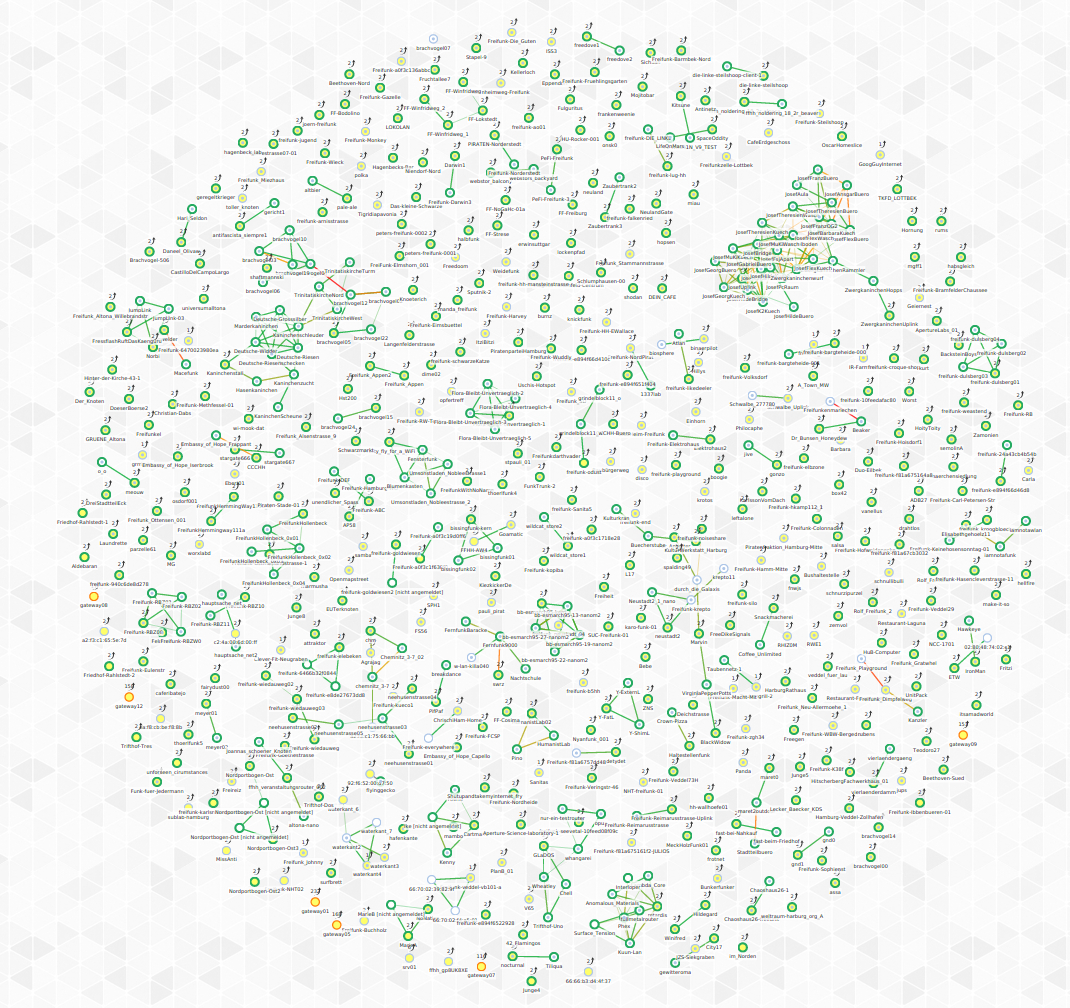
\includegraphics[height=0.8\textheight]{hamburg-graph}
\end{center}
\end{frame}

\section{Solution: Divide \& Conquer}
\begin{frame}{The Winning Strategy\texttrademark}
\begin{center}
\vfill
\pause

\includegraphics[height=0.35\textheight]{cat_tank}$\;$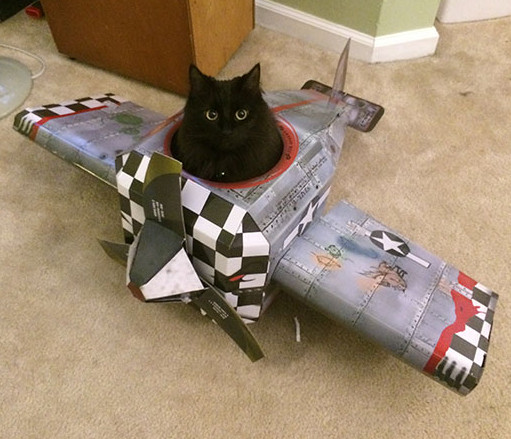
\includegraphics[height=0.35\textheight]{airplane}$\;$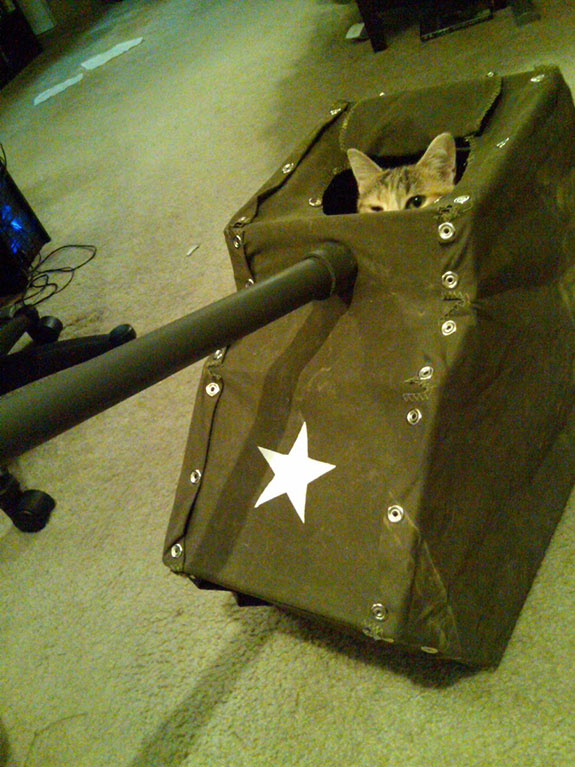
\includegraphics[height=0.35\textheight]{cat_tank2}
\vfill
\Large{Divide \& Conquer!}\end{center}
\vfill
\begin{itemize}
\pause\item We focus on a few city sectors which already have nodes
\pause\item For each sector there will be 1-2 Freifunk representatives
\end{itemize}
\end{frame}

\begin{frame}{The first campaign:}
\begin{center}\Large ``The Long Night of the Freefunkies''\end{center}
\vfill
\begin{itemize}
\pause\item We organize a talk in every sector (at a café, school, etc)
\pause\item All the talks happen at the same time
\pause\item Let's define a date in... November?
\vfill
\pause\item Each local team finds a suitable location
\pause\item I provide slides, teams present them
\pause\item Don't panic! We practice beforehand :)
\pause\item Advertise massively:
\begin{itemize}
\pause\item Globally, in the press and radio
\pause\item Locally: bomb own sector with flyers
\end{itemize}
\end{itemize}
\pause\begin{flushright}
\vspace{-3.35cm}
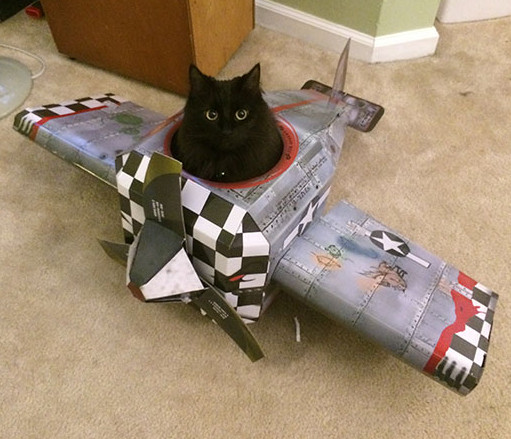
\includegraphics[height=0.3\textheight]{airplane}
\\ \textit{\tiny Bomber cat approves of this!$\quad$}
\end{flushright}
\end{frame}

\section{The sectors}
\begin{frame}{The sectors}
\begin{itemize}
\item I've picked some areas where we already have nodes
\pause\item Not all areas have many public spaces, but we should connect the dots anyway
\pause\item If you want to take care of another area, let me know
\end{itemize}
\end{frame}

\subsection{Johannesviertel}
\begin{frame}{Johannesviertel}
\begin{center}
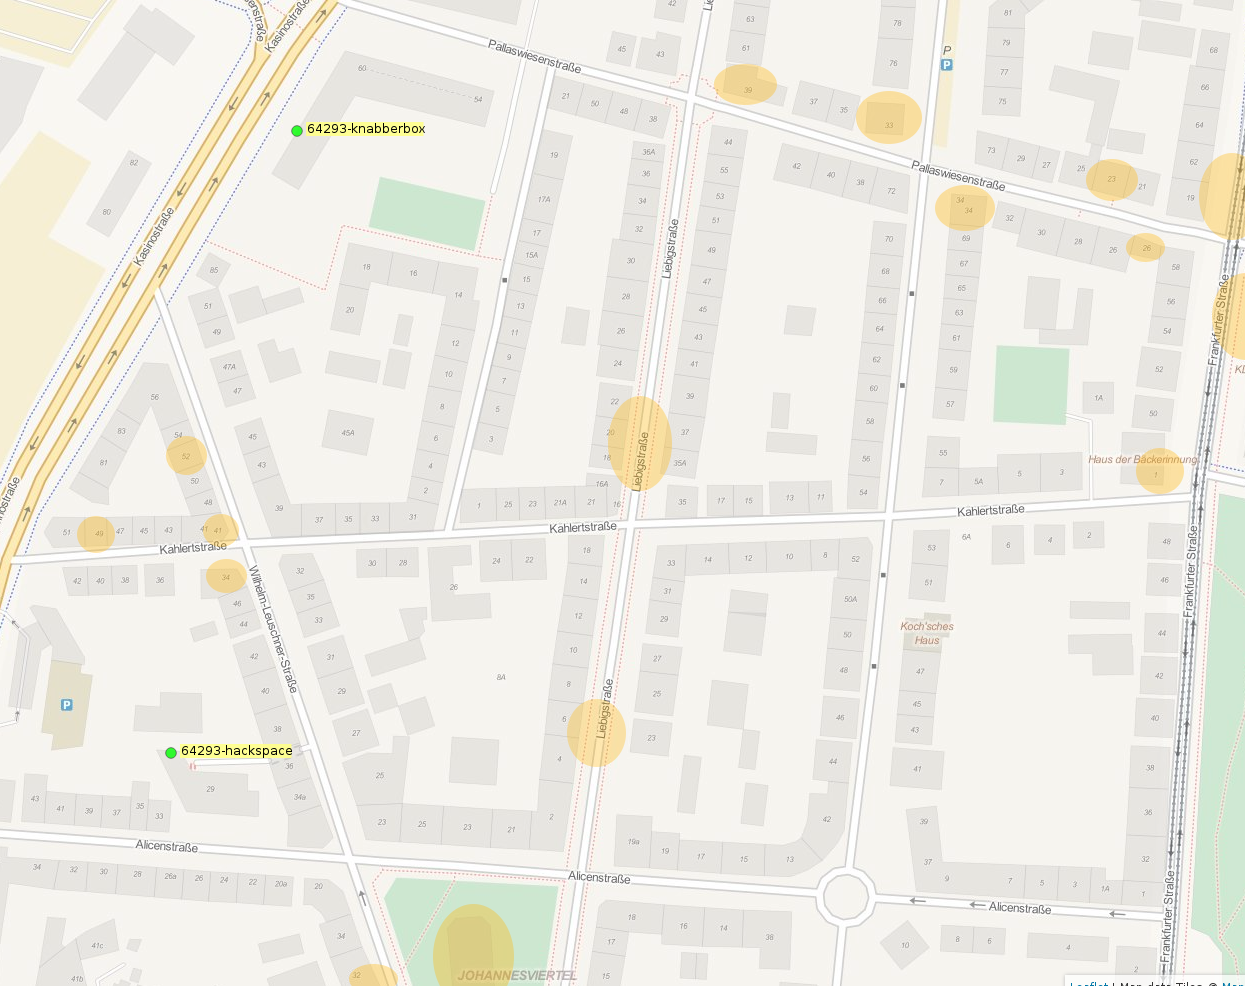
\includegraphics[height=0.8\textheight]{johannesviertel2}
\end{center}
\end{frame}

\subsection{K6}
\begin{frame}{K6}
\begin{center}
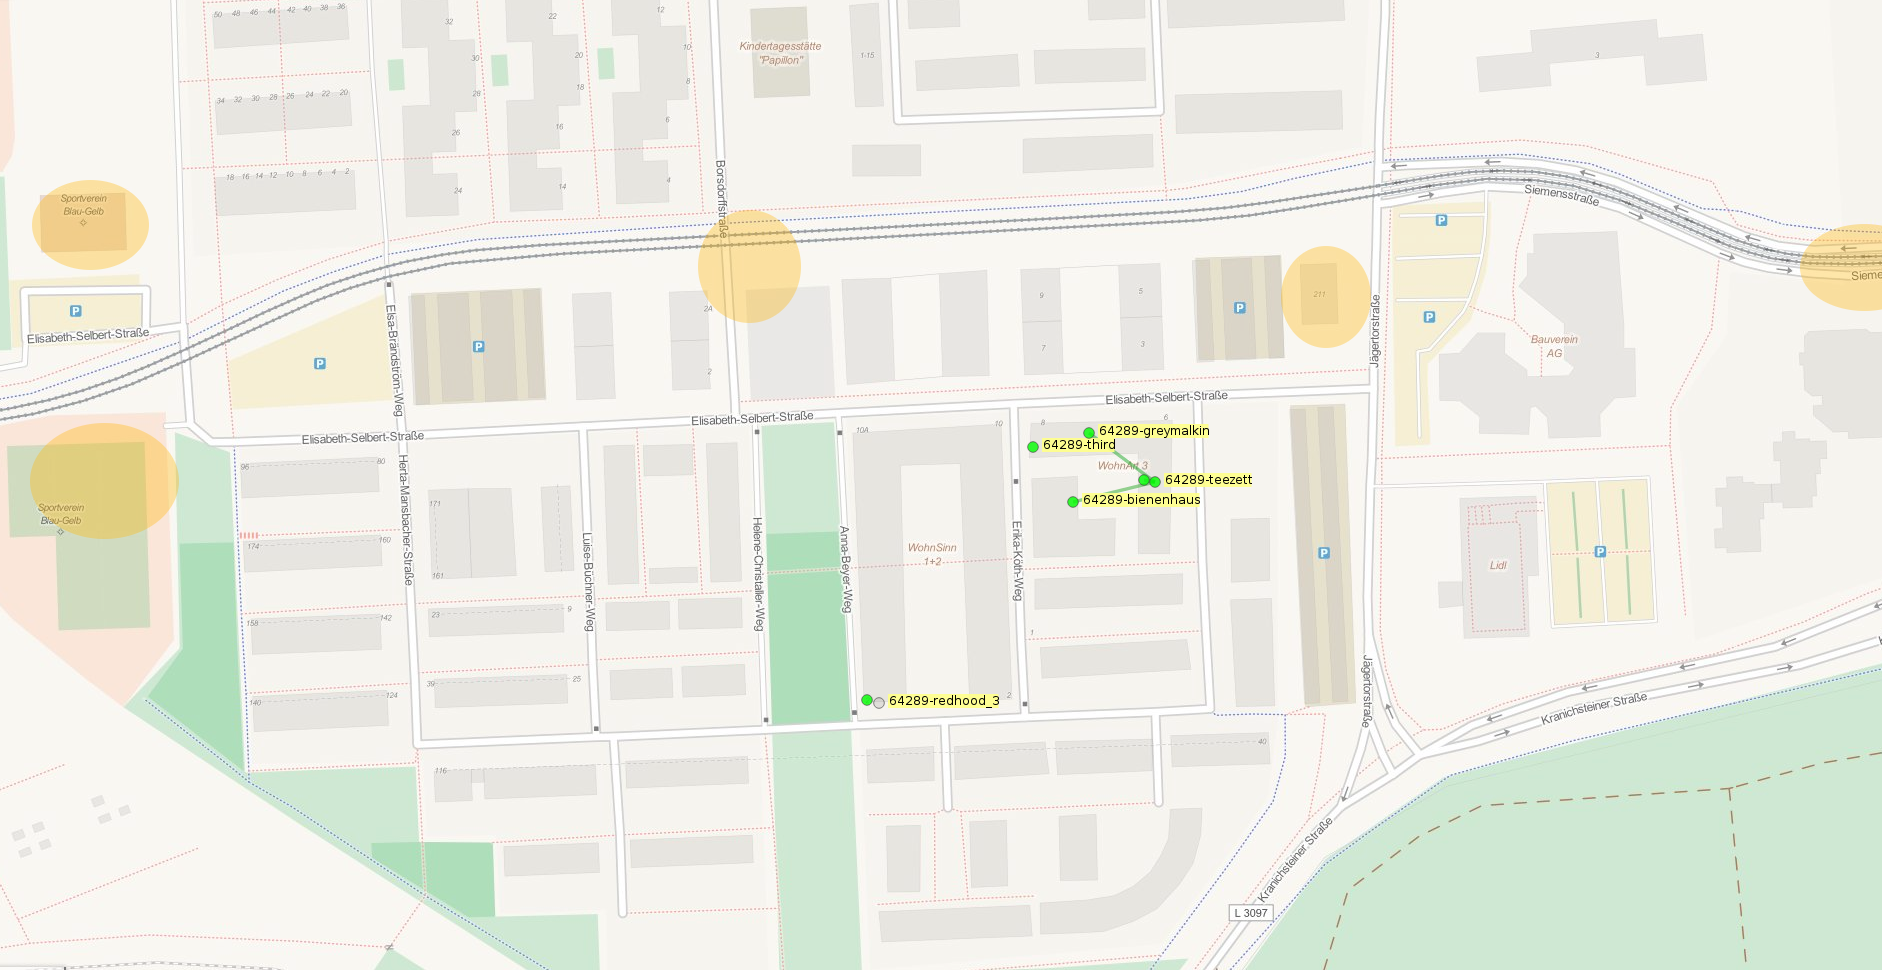
\includegraphics[width=\textwidth]{k62}
\end{center}
\end{frame}

\subsection{Karlshof}
\begin{frame}{Karlshof}
\begin{center}
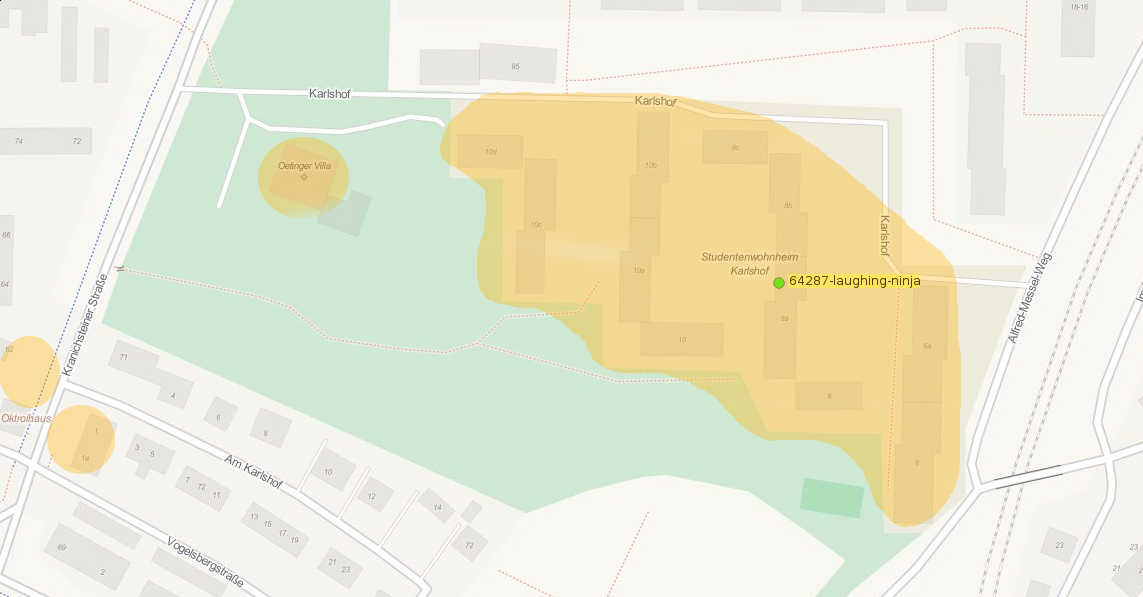
\includegraphics[width=\textwidth]{karlshof2}
\end{center}
\end{frame}

\subsection{Mathildenhöhe}
\begin{frame}{Mathildenhöhe}
\begin{center}
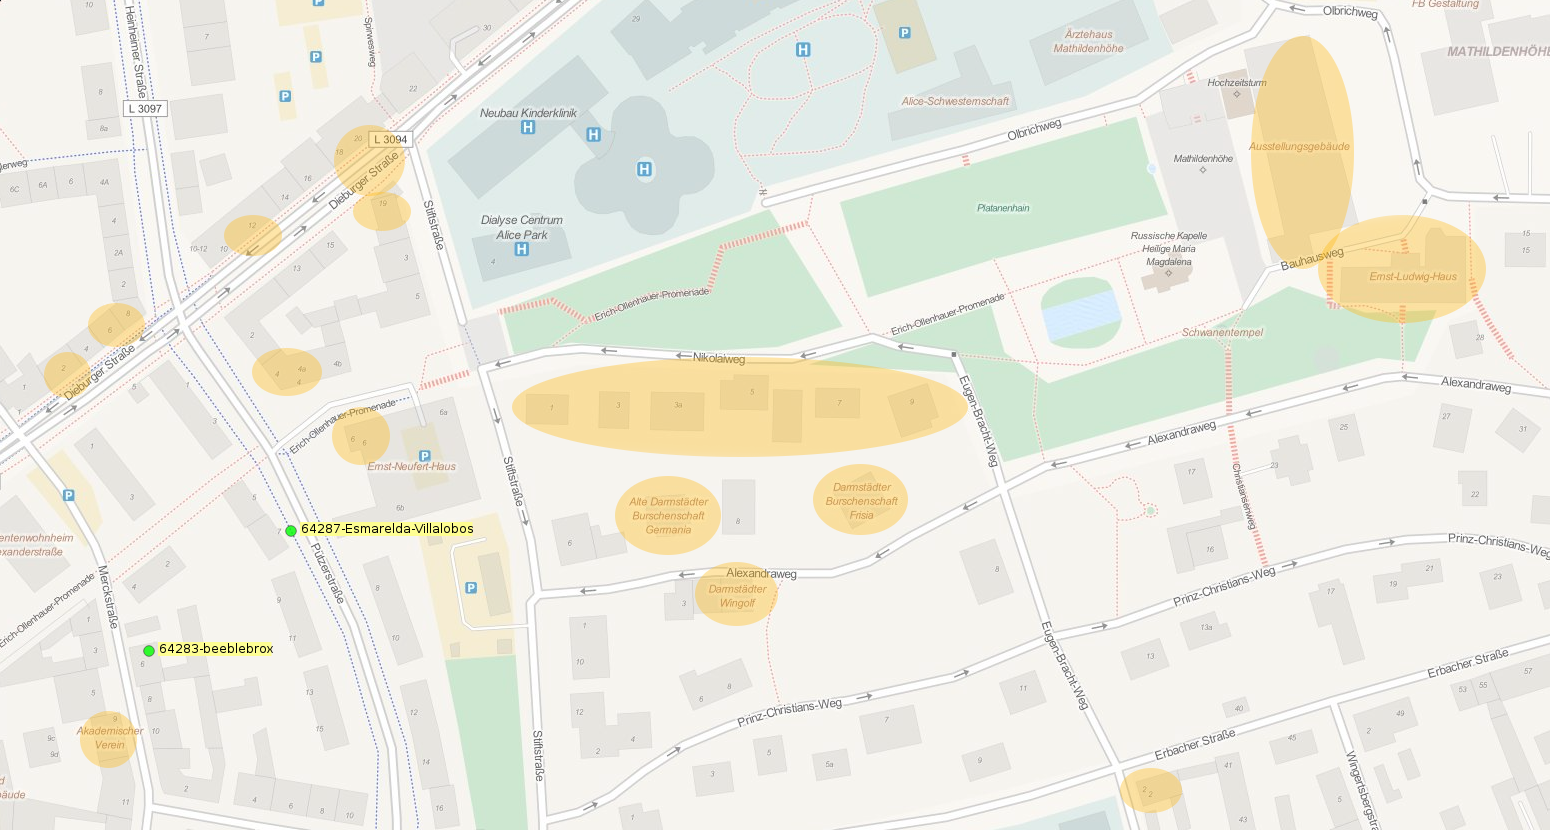
\includegraphics[width=\textwidth]{mathildenhoehe2}
\end{center}
\end{frame}

\subsection{Paulusviertel}
\begin{frame}{Paulusviertel}
\begin{center}
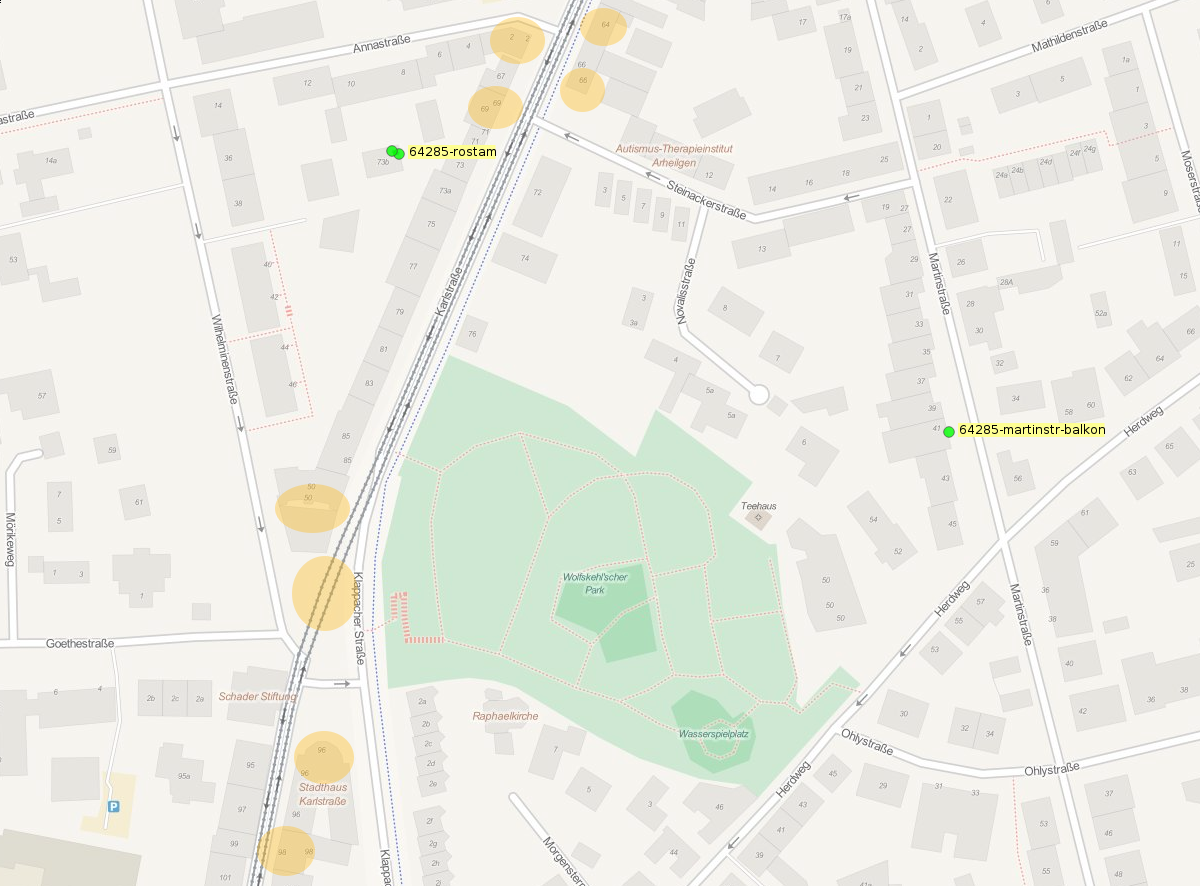
\includegraphics[height=0.8\textheight]{paulusviertel2}
\end{center}
\end{frame}

\subsection{Rhönring/Martinsviertel}
\begin{frame}{Rhönring/Martinsviertel}
\begin{center}
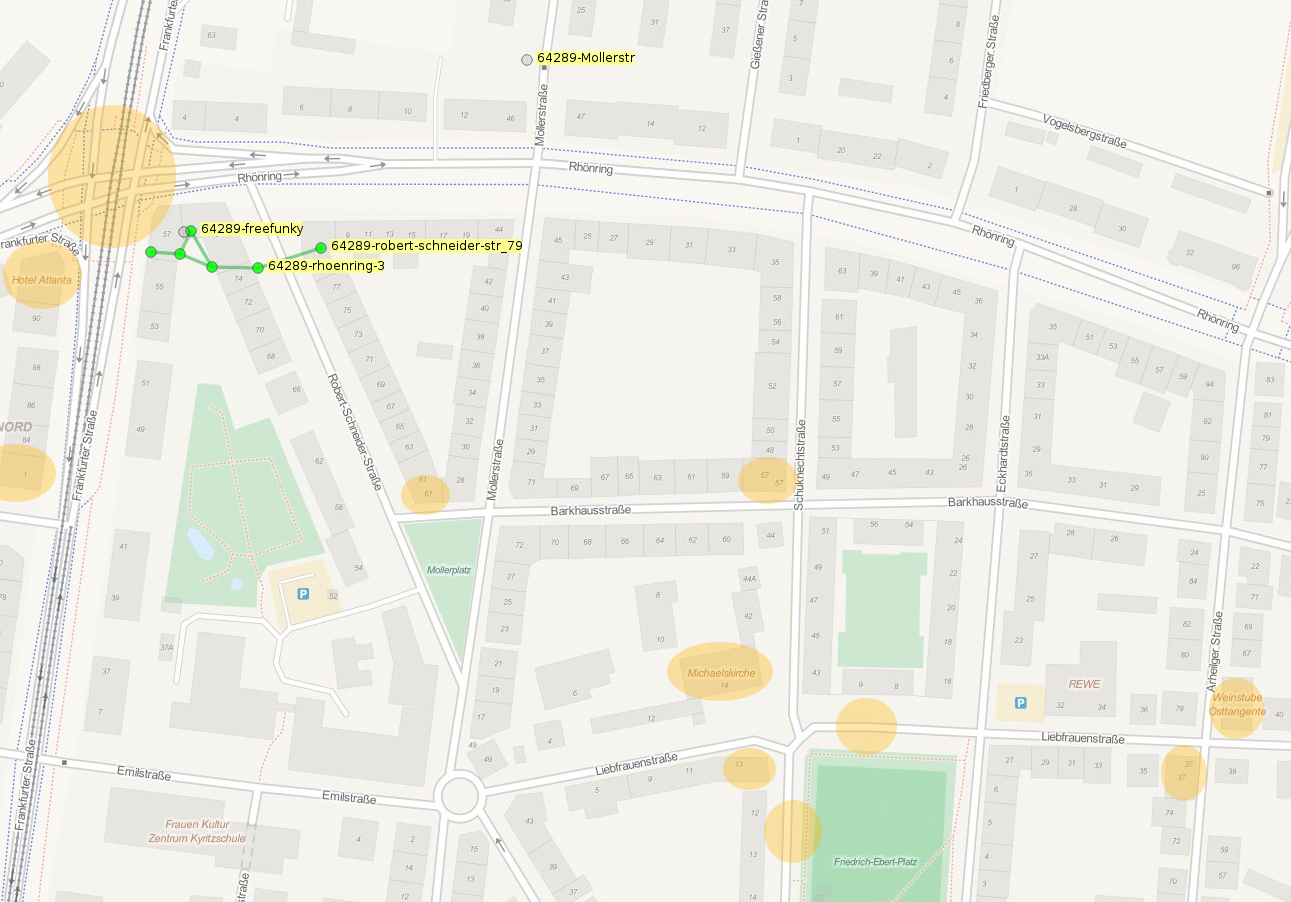
\includegraphics[width=\textwidth]{rhoenring2}
\end{center}
\end{frame}

\subsection{Studentenwohnheim Nieder-Ramstädter-Straße}
\begin{frame}{Studentenwohnheim Nieder-Ramstädter-Straße}
\begin{center}
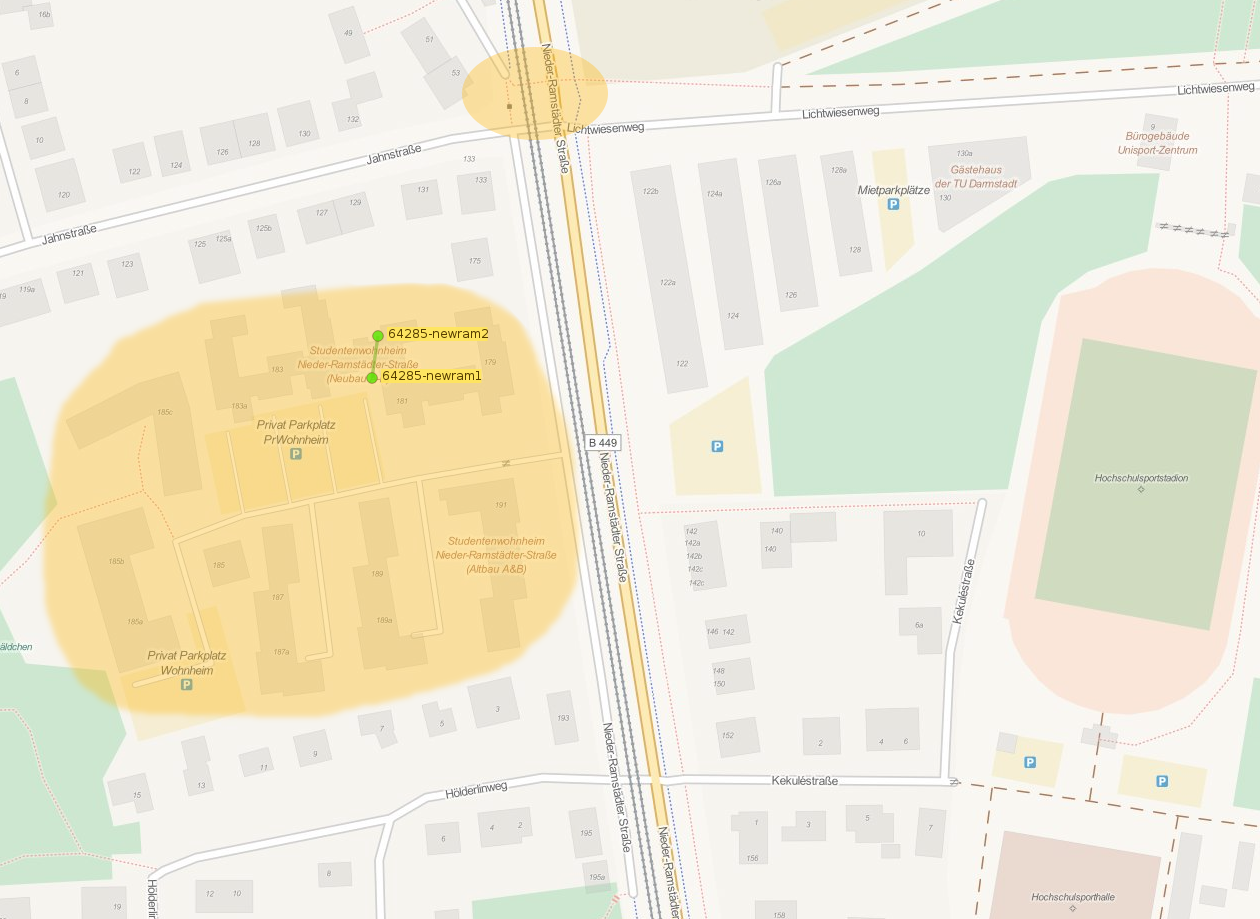
\includegraphics[height=0.8\textheight]{studwohn-nr2}
\end{center}
\end{frame}

\subsection{Südwest}
\begin{frame}{Südwest}
\begin{center}
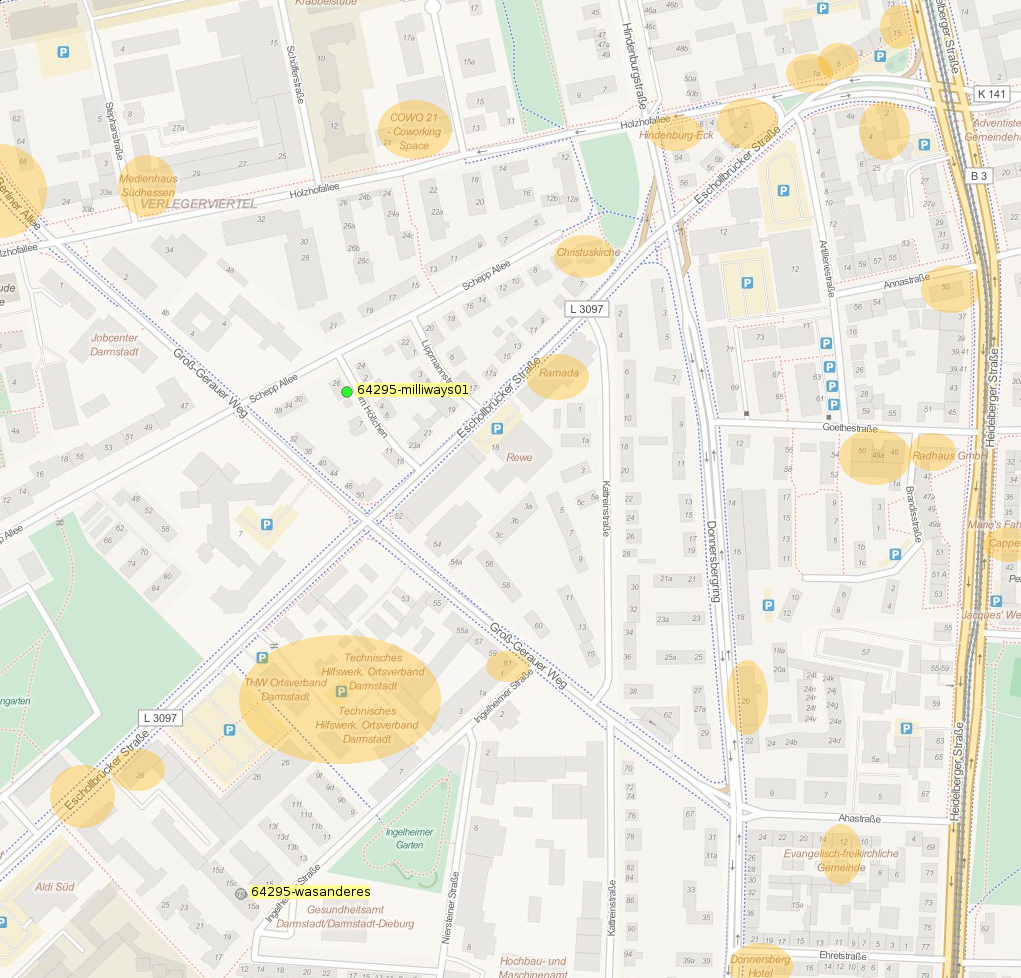
\includegraphics[height=0.8\textheight]{suedwest2}
\end{center}
\end{frame}

\subsection{Woogsviertel}
\begin{frame}{Woogsviertel}
\begin{center}
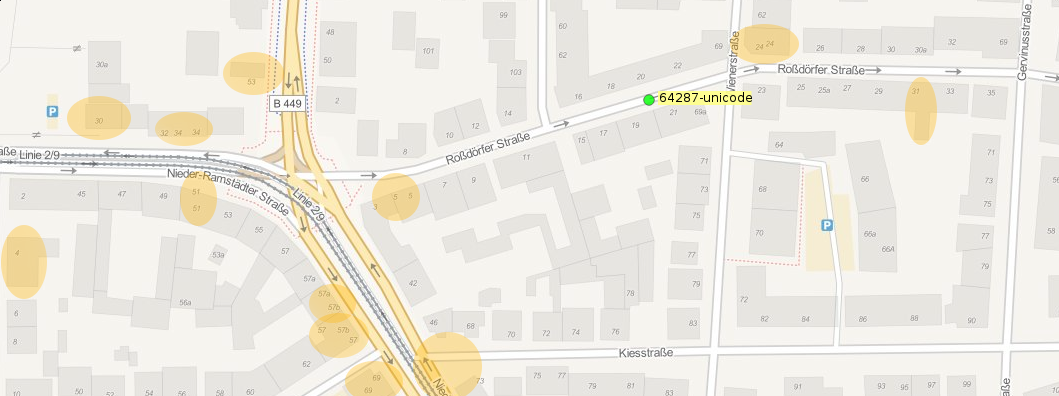
\includegraphics[width=\textwidth]{woogsviertel2}
\end{center}
\end{frame}

\subsection{Zentrum}
\begin{frame}{Zentrum}
\begin{center}
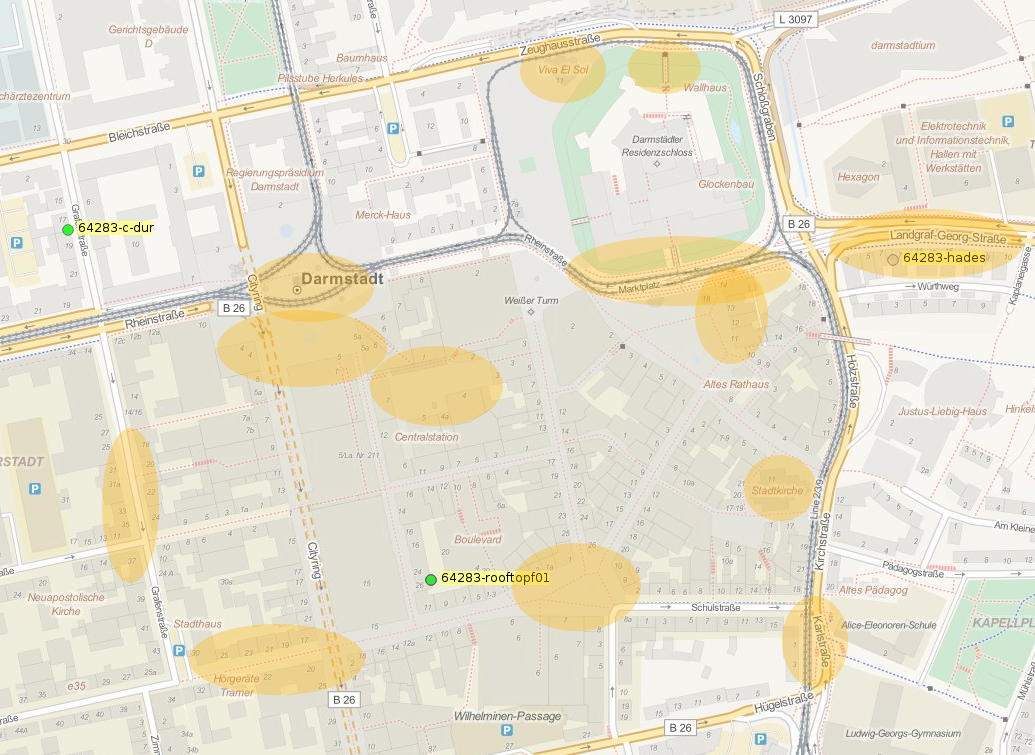
\includegraphics[height=0.8\textheight]{zentrum2}
\end{center}
\end{frame}

\begin{frame}{Target scenario}
\begin{center}
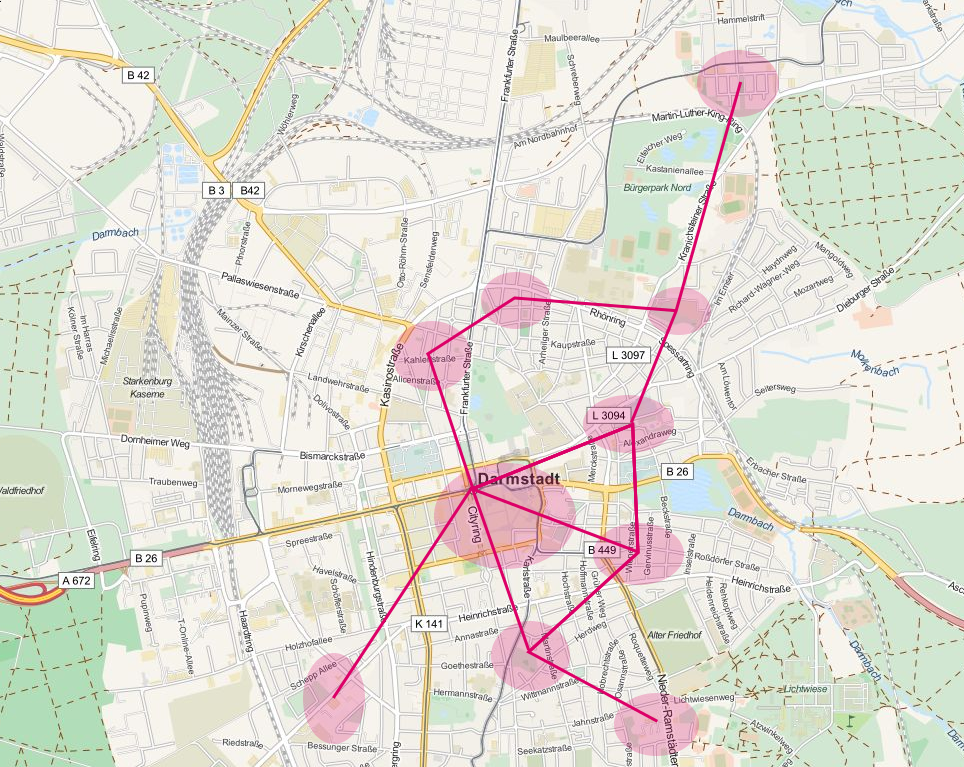
\includegraphics[height=0.8\textheight]{target}
\end{center}
\end{frame}

\begin{frame}{The End}
\vfill
\centering

\includegraphics[width=0.7\textwidth]{mehro} \\
Can haz not disappoint!
\vfill
\end{frame}


\end{document}
